\documentclass[12pt]{article}
\usepackage[top=1in, bottom=1in, left=1in, right=1in]{geometry}

\usepackage{setspace}
\onehalfspacing

\usepackage{amssymb}
\usepackage{amsthm}
\usepackage{epsfig}
\usepackage{times}
\renewcommand{\ttdefault}{cmtt}

\usepackage{amsmath}
\usepackage{graphicx} 
\usepackage{tikz} 
\usepackage{float} 
\usepackage{xspace}
\usepackage{mathrsfs}
\usepackage[mathcal]{euscript}
\usepackage{color}
\usepackage{array}
\usepackage[pdftex,hidelinks]{hyperref}
\usepackage[parfill]{parskip}
\usepackage{multicol}
\usepackage{enumitem}
\usepackage{etoolbox}
\usepackage{subcaption}
\usepackage{cite}
\usepackage{titlesec}
\usepackage[capitalize,compress]{cleveref}

\patchcmd{\thebibliography}{\section*{\refname}}{}{}{}
\titleformat*{\section}{\Large\bfseries}
\titleformat*{\subsection}{\large\bfseries}
\titlespacing{\section}{0pt}{0pt plus 2pt minus 2pt}{0pt plus 2pt minus 2pt}
\titlespacing{\subsection}{0pt}{\parskip}{-\parskip}

% math syntax
\newcommand{\rvec}{\ensuremath{\vec{r}}}
\newcommand{\vecr}{\ensuremath{\vec{r}}}
\newcommand{\vecx}{\ensuremath{\vec{x}}}
\newcommand{\vecy}{\ensuremath{\vec{y}}}
\newcommand{\omvec}{\ensuremath{\hat{\Omega}}}
\newcommand{\vOmega}{\ensuremath{\hat{\Omega}}}

%%%%%%%%%%%%%%%%%%%%%%%%%%%%%%%%%%
%%%%%%%%%%%%%%%%%%%%%%%%%%%%%%%%%%
%%%%%%%%%%%%%%%%%%%%%%%%%%%%%%%%%%
%%%%%%%%%%%%%%%%%%%%%%%%%%%%%%%%%%
\begin{document}

%COVER PAGE

\pagenumbering{gobble}

\begin{center}
{-----  COVER PAGE  ----- \vspace{-5pt}\\ Project Narrative} 

{\textit{Application for Funding Opportunity \#DE-FOA-0001414 \\ U.S. Department of Energy}
}\vspace{-20pt}

\setlength{\unitlength}{1in}
\begin{picture}(6,.1) 
\put(0,0) {\line(1,0){6.25}}
\end{picture}
\vspace{10pt}

{---------- Project Title ---------- \vspace{5pt} \\ \bf  NON-CLASSICAL
TRANSPORT THEORY WITH MULTISCALE PATH DISTRIBUTIONS IN REAL-WORLD APPLICATIONS}
\end{center}


\begin{itemize}[noitemsep,topsep=0pt,parsep=-2pt,partopsep=20pt,labelwidth=7.5cm,align=left,
itemindent=7.5cm]
\item[$\bullet$\, Applicant:] 					{\bf ??????????}
\item[\quad Street Address:] 					{\bf ??????????}  
\item[\quad City:] 									{\bf Berkeley}
\item[\quad State:] 								{\bf California}
\item[\quad Zip:] 									{\bf ??????????}\vspace{12pt}
\item[$\bullet$\, Postal Address:] 			{\bf ??????????} 
\item[\quad (line 2)] 								{\bf ??????????}
\item[\quad (line 3)] 								{\bf ??????????}\vspace{12pt}
\item[$\bullet$\, Lead PI name:] 			{\bf Rachel N. Slaybaugh} 
\item[\quad Telephone Number:]			{\bf 570-850-3385}
\item[\quad Email:]									{\bf slaybaugh@berkeley.edu}\vspace{12pt}
\item[$\bullet$\, Administrative Point of Contact Name:] {\bf ??????????}
\item[\quad Telephone Number:]			{\bf ??????????}
\item[\quad Email:]									{\bf ??????????}\vspace{12pt}
\item[$\bullet$\, Funding Opportunity FOA Number:] {\bf DE-FOA-0001414}\vspace{8pt}
\item[$\bullet$\, DOE/Office of Science Program Office:] {\bf ASCR - Adv. Sci.
 Comp. Research}
\item[\quad Topic Area:]							{\bf Applied Mathematics}
\item[\quad Topic Area Program Manager:] {\bf Steven Lee}\vspace{12pt}
\item[$\bullet$\, PAMS Preproposal Tracking Number:] {\bf ??????????}
\end{itemize}

\pagebreak

IF WE MAKE IT COLLABORATIVE THERE IS A COVER PAGE SUPPLEMENT

\pagebreak

%%%%%%%%%%%%%%%%%%%%%%%%%%%%%%%%%%
%%%%%%%%%%%%%%%%%%%%%%%%%%%%%%%%%%
%%%%%%%%%%%%%%%%%%%%%%%%%%%%%%%%%%
%%%%%%%%%%%%%%%%%%%%%%%%%%%%%%%%%%
\pagenumbering{arabic}

\begin{center}
{\bf  NON-CLASSICAL
TRANSPORT THEORY WITH MULTISCALE PATH DISTRIBUTIONS IN REAL-WORLD APPLICATIONS}
\end{center}\vspace{-20pt}

\setlength{\unitlength}{1in}
\begin{picture}(6,.1) 
\put(0,0) {\line(1,0){6.25}}         
\end{picture}


%----------------------------------------------------------------------
%----------------------------------------------------------------------

\section{Introduction}
We propose to establish and formalize the mathematical foundation of a novel homogenization approach known as \textit{non-classical transport} \cite{larvas11,davxu14,vaslar14a,xudav16}, which will enable better mathematical and computational modeling of particle and radiation transport calculations in heterogeneous random media.
The main impact of this work will be on improving the modeling of transport processes in general three-dimensional (3D) stochastic systems.
We will develop a methodology that will allow us to accurately solve coupled multiscale transport problems in highly heterogeneous systems.
We will also develop an approach to quantify uncertainty with respect to the particular homogenization of the medium.

Accurately modeling transport processes in optical media is integral to several real-world applications that are in line with the goals of the Department of Energy (DOE) and the Advanced Scientific Computing Research (ASCR) program.
These include radiative transfer in the Earth's cloudy atmosphere (see \cite{davxu14,xudav16}, and references therein), neutron transport in certain types of nuclear reactors (see \cite{fragre11,vaslar14b}, and references therein), and computational graphics (CG) rendering (see \cite{yueiwa10,deon14}, and references therein).
Due to the complexity of these systems, spatial variations are often represented with stochastic models.

There are many ways to address stochastic spatial variability in a transport medium; a widely-used and natural approach is \textit{homogenization} \cite{dumgol00,cailac00}.
In this approach, the solution of the transport problem in the heterogeneous stochastic medium is accurately predicted by solving a transport problem in an uniform medium.
Current approaches to homogenize and model particle transport in these applications fail to properly capture important physical aspects of the system \cite{larvas11,davxu14,xudav16,vaslar14b,vas13}.

In this project, we will focus in particular on addressing the challenges involved in modeling transport processes in atmospheric clouds.
The ability to do that accurately in the cloudy atmosphere is crucial to climate modeling research. 
This has been pointed out in a recent report\cite{ipcc13} by the Intergovernmental Panel on Climate Change (IPCC), which states (p. 53) that
\begin{quote}
\textit{``The uncertainty in the WMGHG RF\footnote{Well-mixed greenhouse gas radiative forcing} is due in part to its radiative properties but mostly to the full accounting of atmospheric radiative transfer including clouds''.}
\end{quote}

Moreover, this has been identified by the Exascale Mathematics Working Group as a key area of interest for ASCR research \cite{amrec14}.
On the subject of developing new mathematical tools to address climate models, their report says that (p. 6)   
\begin{quote}
\textit{``... models based on a Markovian assumption will not be adequate.
Models that can represent the physics across a range of scales are likely to be stochastic and include memory effects''}.
\end{quote} 
This is exactly what our proposed work does: it includes a memory variable (the free-path of the particle) to preserve important physical aspects of the stochastic system. 

In addition, we will establish an interdisciplinary collaboration in the field of computer graphics.
Incorporating non-classical free-paths in volume-rendering algorithms will produce more realistic images, as deep penetration of photons is a key feature of high albedo media.
Since this is what happens in atmospheric clouds, we will study the impact of the proposed model in CG rendering.
We will make use of the synergy between these two applications to develop novel approaches, which will provide many insights to both communities.

Finally, we point out that the work we propose will open new research avenues in vital areas of interest for the Applied Mathematics topic area of the ASCR program.
These include, but are not limited to, the implementation of novel computational methods for solving the differential and integro-differential equations involved; studies in uncertainty quantification; innovations in computing large systems of linear equations; and the development of coupled multiscale models.
In short, this work supports the Applied Mathematics goal to solve problems of interest with greater accuracy by more accurately capturing the physics.

In the following sections we will describe the work we will undertake, why it will contribute to advancing the knowledge and understanding of transport problems in stochastic media, and how we will complete the objectives of the proposal.
We start with a discussion on the classical approach used by current tools and why it is insufficient to accurately model non-classical particle transport in relevant applications.
This will be followed by a description of the non-classical theory and a discussion of 
how it will improve our ability to accurately model these problems.
Finally, a detailed research plan describing project execution, milestones, deliverables, and responsibilities is described.

%----------------------------------------------------------------------
%----------------------------------------------------------------------
\section{The Challenge}

We define the free-path $s$ as the distance traveled by a particle (neutron or photon) since its previous interaction (birth or scattering event).
In this definition, the instant after a particle is born or scatters, its value of $s$ is 0. 
In the classical theory of linear particle transport, the incremental probability $dp$ that a particle at point $\rvec = (x,y,z)$ with energy $E$ will experience an interaction while traveling an incremental distance $ds$ is given by $\Sigma_t(\rvec,E)ds$.
Here, the total cross section $\Sigma_t$ is independent of the free-path $s$ and of the direction of flight $\omvec = (\Omega_x,\Omega_y,\Omega_z)$, where $|\omvec|=1$.

Let us consider a single volume of Poisson-distributed (spatially uncorrelated) scattering centers (\cref{fig1}).
\begin{figure}[hbt]
    \centering
    \begin{subfigure}{0.2\textwidth}
        \centering
        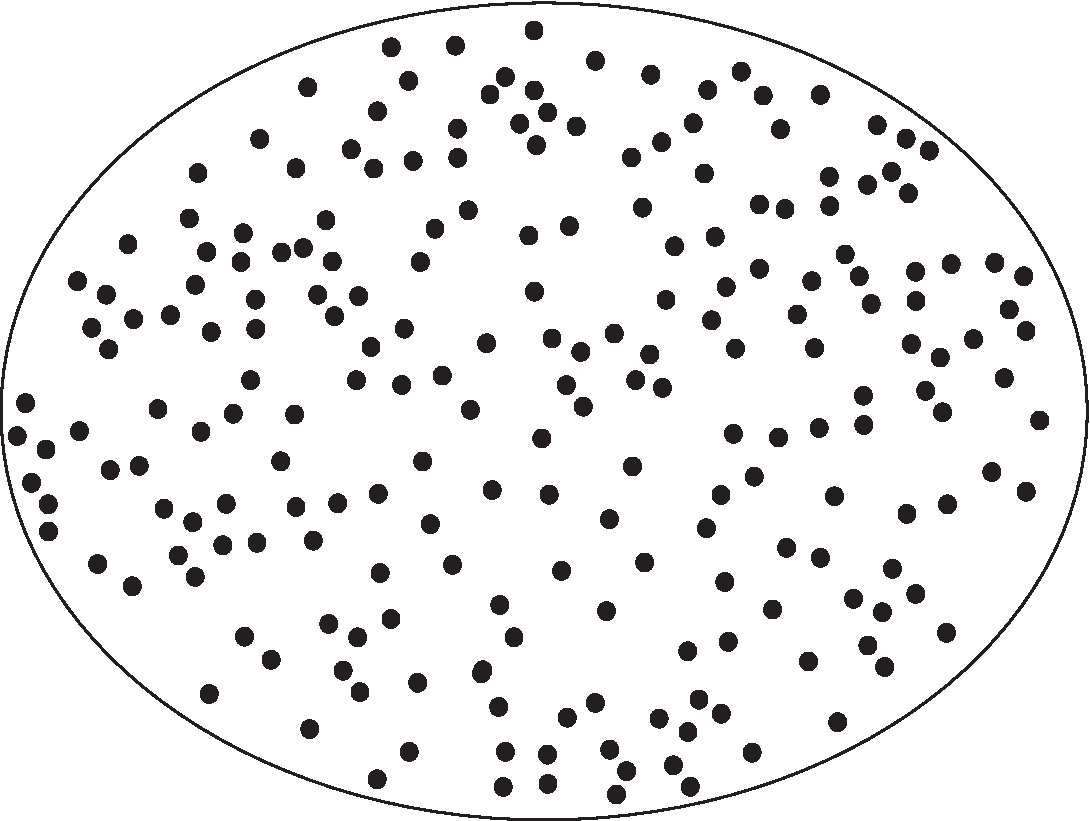
\includegraphics[width=\textwidth]{Fig1a}
    \end{subfigure}
 \caption{Sketch of a volume region containing Poisson-distributed scattering centers.}
    \label{fig1}
\end{figure}
Particles that enter such a volume will undergo many collisions before exiting from it. The probability density function describing the distribution of free-paths within this volume obeys the Beer-Lambert law, and is represented by the exponential
\begin{align}\label{eq1}
p(s) = \Sigma_t e^{-\Sigma_t s}.
\end{align}
Now consider a much larger system formed by randomly placing many of these volumes in a backround ``void'', as sketched in \cref{fig2}.
\begin{figure}[hbt]
    \centering
    \begin{subfigure}{0.3\textwidth}
        \centering
        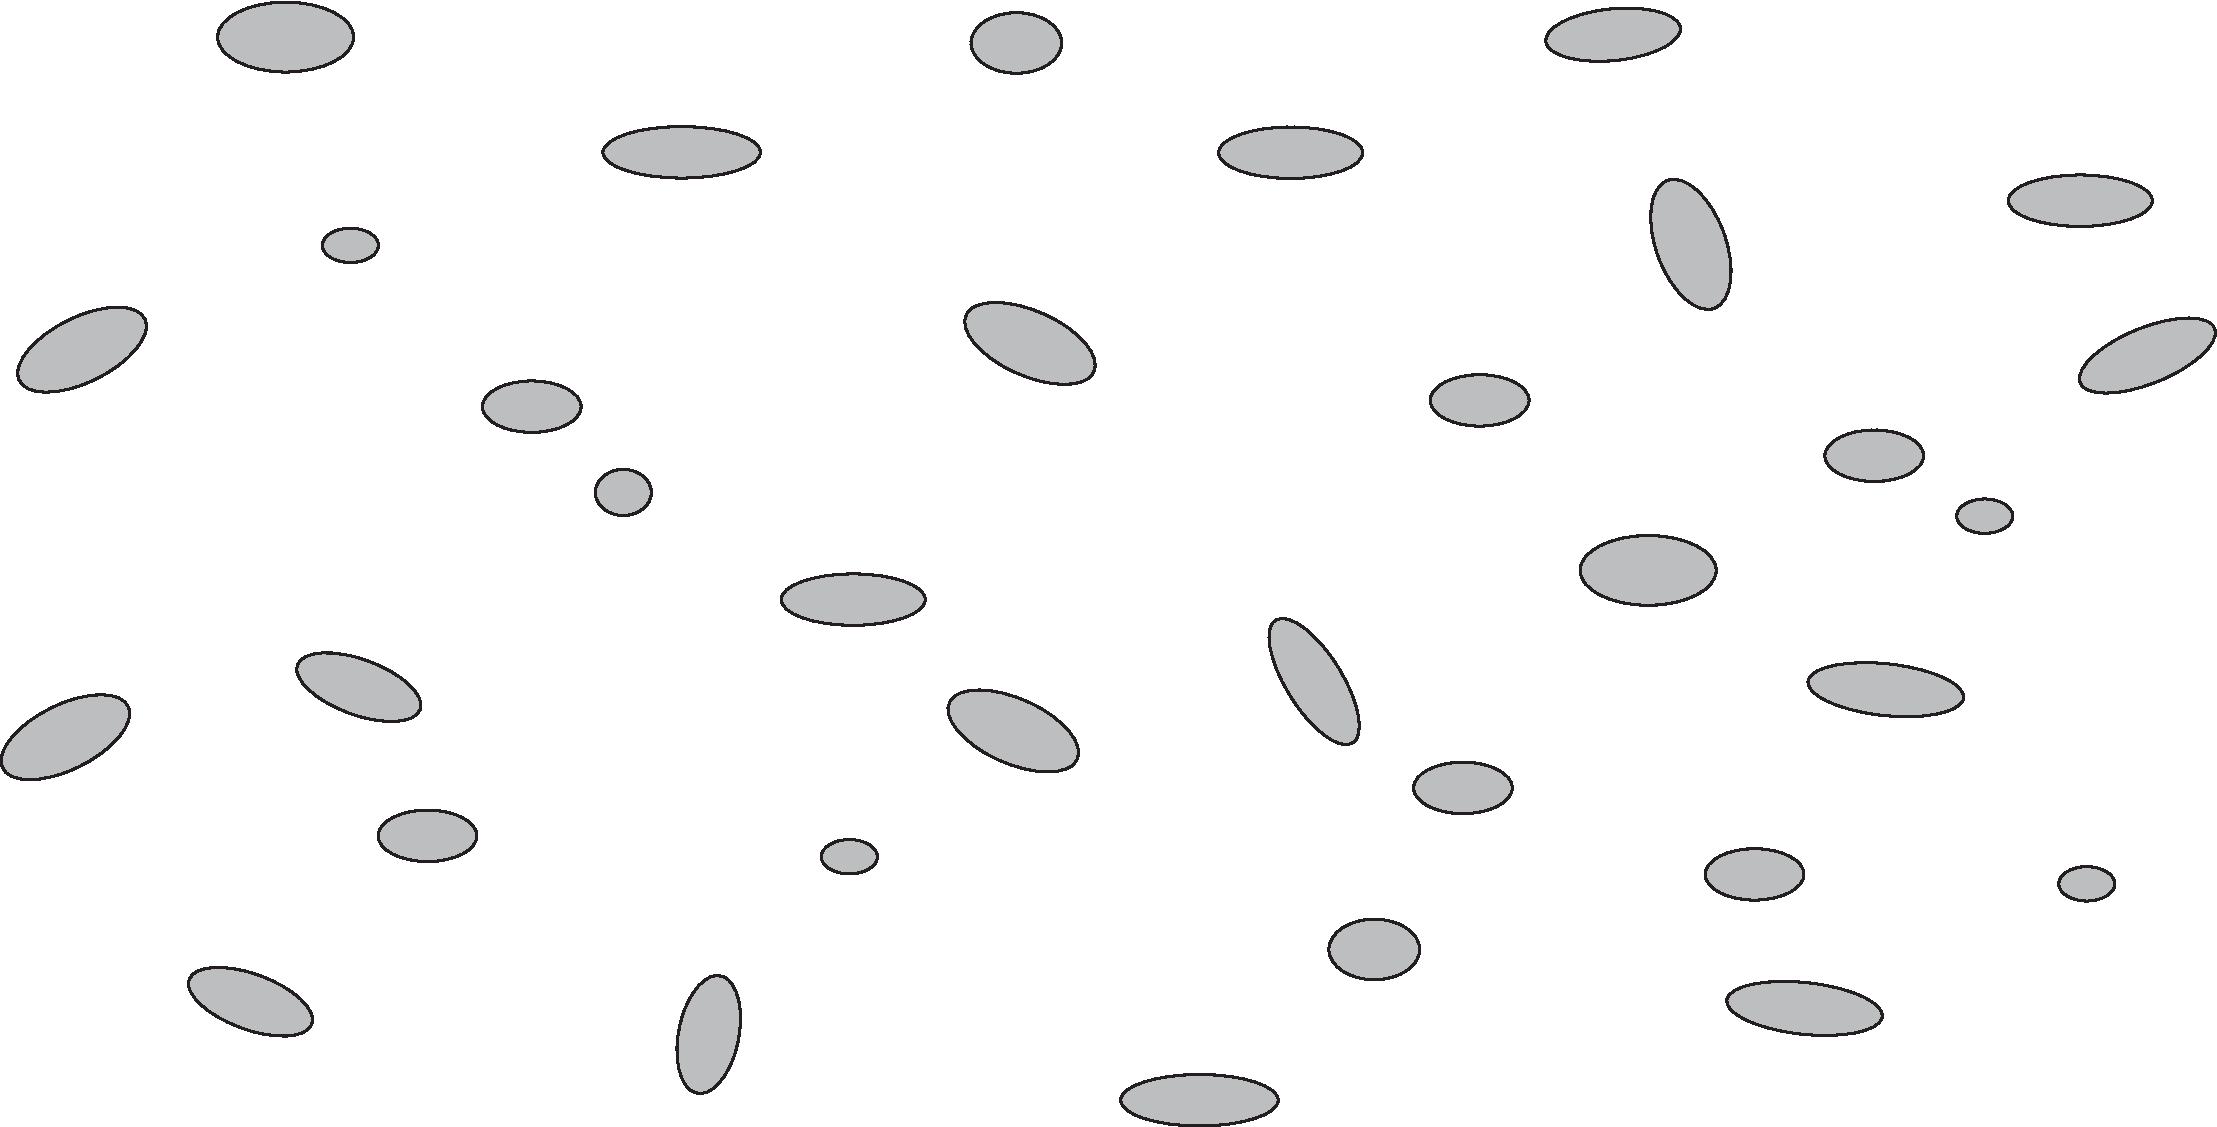
\includegraphics[width=\textwidth]{Fig2a}
    \end{subfigure}
    \caption{Heterogeneous random system formed by many volumes suspended in a void.}
    \label{fig2}
\end{figure}
Notice that the volume regions in this system can be interpreted as water droplets in a cloud, with each point within a water droplet being a potential scattering center.
This type of clumpy medium is also present in Pebble Bed Reactors (PBRs) \cite{fragre11,vaslar14b}, where the volume regions represent the fuel pebbles in the reactor core, with thousands of them piled on top of one another in a random manner.

It is common to use a homogenization model to address transport problems in this kind of random system.
This type of approach seeks to develop effective material properties that can be used in the solution of a transport problem for a uniform medium, while achieving an accurate prediction of the flux behavior in the heterogeneous stochastic medium.
Nevertheless, standard homogenization techniques inherently assume that \cref{eq1} holds in the homogenized material; that is, they assume that the free-path distribution in the uniform medium is given by an exponential (classical transport).  

However, the assumption that $\Sigma_t$ is independent of $s$ is not valid when the locations of the volume regions in the system are correlated.
This correlation leads to a \textit{non-exponential} free-path distribution $p(s)$; we refer this type of transport processes \textit{non-classical}.
The classical homogenization approaches used to address these problems are not capable of preserving the true non-exponential attenuation law that arises in these heterogeneous systems \cite{larvas11,davxu14,vaslar14b,xudav16,vas13}.
This leads to unreliable estimates of the particle flux in these applications, due to important physical quantities being poorly approximated. 

The challenge is to develop and implement a methodology that (i) determines the true free-path distribution in these systems, and (ii) uses that information in a model that preserves the physics of these stochastic processes.
To do that, we will use a novel theory specifically developed to address non-classical transport.   

%----------------------------------------------------------------------
%----------------------------------------------------------------------
\section{The Non-classical Theory}

To address the challenges of modeling systems with non-exponential particle attenuation, a generalization of the linear Boltzmann equation has been developed \cite{larvas11,davxu14,vaslar14a,xudav16}.
The generalized equation assumes that the positions of the scattering centers are correlated but independent of direction $\omvec$.
For the sake of simplicity, let us consider monoenergetic transport with isotropic scattering; in this case, the \textit{non-classical transport equation} can be written as
\begin{align}
\frac{\partial \psi}{\partial s}(\rvec,\omvec,s) + \omvec\cdot\nabla\psi(\rvec,\omvec,s) &+ \Sigma_t(s)\psi(\rvec,\omvec,s)\label{eq2} \\
=
&\frac{\delta(s)}{4\pi}\left[c\int_{4\pi}\int_0^\infty \Sigma_t(s')\psi(\rvec,\omvec',s')ds'd\Omega' + Q(\rvec)\right],\nonumber
\end{align}
where $\psi$ is the non-classical angular flux, $c$ is the scattering ratio (such that the scattering cross section $\Sigma_s = c\Sigma_t$), and $Q$ is an isotropic source.
Here, the non-classical homogenized total cross section $\Sigma_t(s)$ is defined such that
\begin{align*}
\Sigma_t(s)ds =
\begin{array}{l}
\text{the probability that a particle that has traveled
a distance $s$ since its previous}\\
\text{interaction (birth as a source particle or scattering event) will experience its}\\
\text{next interaction while
traveling a further distance $ds$,}
\end{array}
\end{align*}
and we can obtain the classical angular flux $\Psi(\rvec,\omvec)$ by computing
\begin{align}
\Psi(\rvec,\omvec) = \int_0^\infty \psi(\rvec,\omvec,s)ds.
\end{align}
The generalized model described by \cref{eq2} effectively homogenizes the heterogeneous media by including the memory variable $s$ and by incorporating its \textit{true} (non-exponential) free-path distribution $p(s)$, which is related to the non-classical cross-section by \cite{larvas11}
\begin{align}\label{eq4}
p(s) = \Sigma_t(s)\exp\left[-\int_0^s\Sigma_t(s')ds'\right].
\end{align}
Notice that, if $\Sigma_t(s)=\Sigma_t$ is independent of $s$, \cref{eq4} reduces to \cref{eq1}, and \cref{eq2} reduces to the classical transport equation
\begin{align}\label{eq5}
\omvec\cdot\nabla\Psi(\rvec,\omvec) + \Sigma_t\Psi(\rvec,\omvec)
= \frac{1}{4\pi}\left[c\int_{4\pi} \Sigma_t\Psi(\rvec,\omvec')d\Omega' + Q(\rvec)\right].\nonumber
\end{align}
Existence and uniqueness of solutions have been rigorously discussed in \cite{fragou10}.
The non-classical theory was extended in \cite{vaslar14a} to include angular-dependent free-path distributions in order to investigate anisotropic diffusion of neutrons in 3D PBR cores.
A similar kinetic equation with free-path as an independent variable has been rigorously derived for the periodic Lorentz gas in a series of papers by Golse and colleagues (cf. \cite{gol12} for a review), and by Marklof \& Str\"ombergsson (cf. \cite{marstr11,marstr15}). 

%----------------------------------------------------------------------
%----------------------------------------------------------------------
\section{Related Preliminary Results}

We have already shown that the classical linear Boltzmann equation and diffusion-based approximations are particular cases of the non-classical equation \cite{frakry15,vas16}.
Moreover, one can combine moment methods and the Fourier transform to derive fractional diffusion equations from the non-classical transport equation \cite{frasun16}.
This is key to model radiative transfer problems in atmospheric clouds, where generalized (anomalous) diffusion arises due to long-tailed free-path distributions. 

With respect to Pebble Bed Reactors, non-classical methods have been shown to outperform current homogenization techniques in diffusive systems \cite{larvas11,vaslar14b,vas13} and in certain types of one-dimensional (1D) transport problems \cite{vaskry16}.   
Moreover, ****INTERESTING RADIATIVE TRANSFER RESULT (FIGURE / TABLE)***
\begin{center}
*****PLACEHOLDER FOR EXAMPLE OF RADITIVE TRANSFER RESULTS*****
\end{center} 
These preliminary numerical results offer a strong case for the non-classical theory, and justify the efforts to develop and improve related tools.

However, results for transport problems in higher dimensions have not yet been performed. The reason is that, in order to solve the non-classical transport equation, one must know the true (ensemble-averaged) free-path distribution function of the system.
Although there are a few particular cases in which an analytical expression for $p(s)$ can be obtained \cite{vaskry16,vassla16}, doing so for general 3D random systems is still far from being achieved.   

%----------------------------------------------------------------------
%----------------------------------------------------------------------
\section{Description of Proposed Research}

%-----------------------------
%-----------------------------
\subsection{Objectives}

This project will focus on advancing the mathematical aspects of the non-classical theory, and on developing a set of computational tools to solve general, 3D non-classical transport problems in real-world applications.
To achieve that, we will build upon the results presented in the last section to expand and improve the mathematical and computational aspects of the non-classical theory.
Moreover, the interdisciplinary scope of the project combined to the different areas of expertise of the team will create perfect conditions to perform cutting-edge research, fostering ideas and driving innovations.

We will leverage computational techniques currently used in CG rendering (cloud modeling) to create a tool that will allow us to numerically estimate the $p(s)$ in general 3D stochastic and heterogeneous systems.
This will enable us to solve the full non-classical transport equation and study its performance in different scenarios, while addressing a number of current challenges in the areas of applied mathematics and engineering.

One of the main features of this approach will be the ability to refine the resolution of the free-path distribution in different regions of interest, allowing us to accurately solve coupled multiscale transport problems in highly heterogeneous systems.
The expectation is that the non-classical approach will be less costly and more accurate than existing methods once it is fully implemented since it preserves important elements of physics that are not captured by the current models.

%-----------------------------
%-----------------------------
\subsection{Path to Success}

We identify \textit{five} key tasks that need to be completed in order to successfully accomplish the proposed work: numerically determining $p(s)$; choosing the transport solver; implementing and validating the method; extending the method to multiscale problems; and measuring the impact.
These are the major steps in the project; the work involved to achieve them will fill gaps in science and engineering research that further DOE-ASCR goals.
We will now describe the approach we will use to fulfill each of these tasks. 

%-----------------------------
%-----------------------------
$\bullet$ \underline{Numerically Determining $p(s)$:}

The initial phase of this work will focus on the development and analysis of the numerical approach to obtain the homogenized free-path distribution $p(s)$ in general, 3D, stochastic and heterogeneous systems.
This will be accomplished by taking full advantage of the team's expert in graphics research.
Tapping into this expertise, we will apply cutting-edge techniques used in volume-rendering algorithms to efficiently tally an accurate numerical estimate of the ensemble-averaged $p(s)$ in these random systems. 

This algorithm will first be implemented in a scoping code for method characterization and investigation.
Determining the best way to obtain the ensemble-averaged $p(s)$ for any stochastic mixture will be the primary challenge of this task; the lessons learned in doing so will be a valuable contribution to the wider scientific community.
We will carry on the mathematical formalization of the methodology, and will analyse methods to quantify the uncertainty arising from the homogenization of $p(s)$ in these systems.

%-----------------------------
%-----------------------------
$\bullet$ \underline{Choosing the Transport Solver}

Once we have developed the algorithm to attain $p(s)$, we need to introduce it into a code to solve the 3D non-classical transport equation.
The choice of solver to use--deterministic or Monte Carlo--is of vital importance for the success of the project; thus, we will thoroughly weigh the pros and cons of each approach.

To do that, we will write preliminary versions of the codes for each solver and apply them to simple transport problems.
We will evaluate the results and carry out a technical assessment, taking into account the accuracy, cost-efficiency, and potential pitfalls identified for each solver, as well as other foreseen issues as we move forward.

First, we will test the non-classical codes by solving \textit{classical} transport problems in homogeneous and heterogeneous systems; this will allow us to validate the methods using standard (classical) solution techniques.
Next, we will solve non-classical problems in specific ``toy'' models, for which either analytical or benchmark solutions exist for a reliable comparison.
We will then have enough the data to make an informed decision.
If early in this process it becomes clear that one of the models strongly outperforms the other, we shall pick that method without having to complete this evaluation.

%-----------------------------
%-----------------------------
$\bullet$ \underline{Implementing and Validating the Method}

Having chosen the transport solver, we can proceed to implement the full computational model.
As we move from the basic transport problems addressed in the previous task to more complex non-classical problems, we need to use different approaches to validate the proposed method.
These will depend on the type of applications/systems being addressed, and will include any combination of benchmark solutions, Monte Carlo simulations of the random system (not homogenized), and experimental results.

We will start by focusing on simple (but important) non-classical problems in real-world climate modeling/remote sensing applications, relying on the team's expertise in this area to choose the best validation technique.
We will then test and validate the proposed model in an expanded set of applications, including other areas in science and engineering where transport in 3D stochastic spatial structures is important.

Finally, we will use the proposed computational model to validate some mathematical aspects of the non-classical theory.
The asymptotic convergence of the non-classical transport equation to simpler representations of the transport process will be examined, and original asymptotic analyses for selected models (e.g.\ simplified P$_N$ equations) will be performed.
We will use the set of tools developed to numerically validate these new results as well as other--already established--asymptotic limits of the non-classical theory (e.g.\ fractional diffusion).

%-----------------------------
%-----------------------------
$\bullet$ \underline{Extending the Method to Multiscale Problems}

After the successful implementation and validation of the proposed model, we will extend the capabilities developed up to this point to create free-path distributions that can accurately capture highly-resolved heterogeneities in small length scales.
This will enable us to ``fine-tune'' the $p(s)$ at different regions of the system, allowing us to effectively describe the non-classical transport process as a multiscale problem.

This gives us a set of coupled multiscale transport equations in the larger system that can be solved without the cost of fine resolution for the $p(s)$ everywhere, while still preserving significant information where needed.
We will perform a thorough sensitivity analysis and will broaden the uncertainty quantification approach used in the first task to include this extended, multiscale homogenization of $p(s)$. 

%-----------------------------
%-----------------------------
$\bullet$ \underline{Measuring Impact}

We will measure the impact of the proposed model by analyzing its performance (accuracy, time, etc.) compared to current homogenization techniques and other non-homogenization approaches.
We will investigate how the choice of the system affects its performance, and what kind of real-world applications are best suited to the non-classical theory.
We will also determine how efficiently this approach models multiscale and multiresolution problems.


%-----------------------------
%-----------------------------
\subsection{Deliverables}

The first deliverable from this project will be a high-quality set of mathematical and computational tools to address non-classical transport problems in general 3D random systems.
These tools will have the capability to accurately and efficiently solve coupled multiscale transport problems in systems with very strong heterogeneities.
They will also contain an approach to quantify the uncertainties that emerge from the non-classical homogenization.

The second deliverable will consist of a series of impact studies on relevant application problems, which will become a powerful demonstration platform for our innovative methods in theoretical and computational transport.
At a minimum, we will pursue radiative transfer in atmospheric clouds, computational graphics, and nuclear reactor core physics.
We will provide a set of results and corresponding analysis from these impact studies using realistic problems;
these will be the first examples of the impact that this new approach can have by incorporating non-classical transport characteristics.

These two deliverables will include an informative and robust test suite and version control of the source code as part of a transparent development process.
Furthermore, we will focus in identifying how the improvements obtained with this new methodology will impact exascale-resolution problems.


%-----------------------------
%-----------------------------
\section{Team Capabilities and Experience}

This research is accomplishable because of the technical quality of the proposed work and the deep experience and strong capability of the applicant team.
Our project team is strongly interdisciplinary, formed by experts in the different areas of the proposed scope:

$\bullet$ Slaybaugh is an Assistant Professor of Nuclear Engineering at UC Berkeley, with experience in deterministic and Monte Carlo radiation transport codes, high-quality software development, and supercomputing.
Her research program is based in computational methods applied to existing and advanced nuclear reactors, nuclear non-proliferation and security, and shielding applications. 

$\bullet$ Vasques is a Project Scientist at UC Berkeley, with experience in mathematical and computational modeling, stochastic processes, and transport theory.
His main area of research is based on modeling transport processes in stochastic mixtures, focusing on non-classical particle transport.

$\bullet$ Davis...

$\bullet$ Wrenninge...

$\bullet$ Frank...


%-----------------------------
%----------------------------- 
\section{Timeline and Responsibilities}

\textcolor{red}{[note: to be deleted] It should also include a timeline for the major activities of the proposed
project, and should indicate which project personnel will be responsible for which activities.
There should be no ambiguity about which personnel will perform particular parts of the project or the time at which these activities will take place.}

The PI will be responsible for
\begin{itemize}[noitemsep]
\item Mentoring and directing the graduate students conducting research
\item Ensuring good coding practices
\item Helping students identify information and venues for presentation and publication of results
\item Meeting all requirements for reports and deliverables to the sponsor
\item Managing and administering awarded funds, assisted by the PI's institution
\end{itemize}

The Co-investigators and Key Personnel will be responsible for
\begin{itemize}[noitemsep]
\item Providing support and input throughout the project
\item Contributing their time and expertise to specific tasks as applicable
\item Providing additional student guidance and mentorship as applicable
\end{itemize}

The following is the project's timeline, identifying the major activities and indicating the responsible personnel:
\begin{itemize}
\item \textit{Year 1}
\begin{itemize}[noitemsep]
\item Numerically determine $p(s)$: Vasques, Wrenninge
\item Begin quantifying uncertainty associated with homogenizing the system: Frank, Vasques
\item Choose the transport solver: Davis, Slaybaugh, Vasques
\item Begin method implementation: Slaybaugh, Vasques
\item Begin identifying impact problem set: Davis, Slaybaugh, Wrenninge
\end{itemize}
\item \textit{Year 2}
\begin{itemize}[noitemsep]
\item Continue quantifying uncertainty associated with homogenizing the system: Frank, Vasques
\item Complete method implementation, conduct associated validation: Slaybaugh, Vasques
\item Finish identifying impact problem set: Davis, Slaybaugh, Wrenninge
\item Begin extending the method to multiscale: Slaybaugh, Vasques, Wrenninge
\end{itemize}
\item \textit{Year 3}
\begin{itemize}[noitemsep]
\item Complete quantifying uncertainty associated with homogenizing the system: Frank, Vasques 
\item Complete extending the method to multiscale: All
\item Conduct impact tests: Davis, Slaybaugh, Vasques
\end{itemize}
\end{itemize}



%%%%%%%%%%%%%%%%%%%%%%%%%%%%%%%%%%
%%%%%%%%%%%%%%%%%%%%%%%%%%%%%%%%%%
%%%%%%%%%%%%%%%%%%%%%%%%%%%%%%%%%%
%%%%%%%%%%%%%%%%%%%%%%%%%%%%%%%%%%
\pagebreak

\pagenumbering{gobble}

\begin{center}
{\bf APPENDIX 3 -- BIBLIOGRAPHY \& REFERENCES CITED} 
\end{center}

\begin{thebibliography}{10}

\bibitem{larvas11}
E.W.~Larsen and R.~Vasques.
``A generalized linear Boltzmann equation for non-classical particle transport.''
\textit{Journal of Quantitative Spectroscopy \& Radiative Transfer} \textbf{112}: 619--631 (2011).\vspace{-5pt}

\bibitem{davxu14}
A.B.~Davis and F.~Xu.
``A generalized linear transport model for spatially correlated stochastic media.''
\textit{Journal of Computational and Theoretical Transport} \textbf{43}: 474--514 (2014).\vspace{-5pt}

\bibitem{vaslar14a}
R.~Vasques and E.W.~Larsen.
``Non-classical particle transport with angular-dependent path-length distributions. I: Theory.''
\textit{Annals of Nuclear Energy} \textbf{70}: 292--300 (2014).\vspace{-5pt}

\bibitem{xudav16}
F.~Xu., A.B.~Davis, and D.J.~Diner.
``Markov chain formalism for generalized radiative transfer in a plane-parallel medium, accounting for polarization.''
\textit{Journal of Quantitative Spectroscopy \& Radiative Transfer} \textbf{184}: 14--26 (2016).\vspace{-5pt}

\bibitem{fragre11}
M.~Fratoni and E.~Greenspan.
``Neutronic feasibility assessment of liquid salt-cooled pebble bed reactors.''
\textit{Nuclear Science and Engineering} \textbf{168}: 1--22 (2011). \vspace{-5pt}

\bibitem{vaslar14b}
R.~Vasques and E.W.~Larsen.
``Non-classical particle transport with angular-dependent path-length distributions. II: Application to pebble bed reactor cores.''
\textit{Annals of Nuclear Energy} \textbf{70}: 301--311 (2014). \vspace{-5pt}

\bibitem{yueiwa10}
Y.~Yue, K.~Iwasaki, B-Y.~Chen, Y.~Dobashi, and T.~Nishita.
``Unbiased, adaptive stochastic sampling for rendering inhomogeneous participating media.''
\textit{ACM Transactions on Graphics} \textbf{29}: \#177 (2010).\vspace{-5pt}

\bibitem{deon14}
E.~d'Eon.
``Rigorous asymptotic and moment-preserving diffusion approximations for generalized linear Boltzmann transport in arbitrary dimension.''
\textit{Transport Theory and Statistical Physics} \textbf{42}: 237--297 (2014).\vspace{-5pt}

\bibitem{dumgol00}
L.~Dumas and F.~Golse.
``Homogenization of transport equations."
\textit{SIAM Journal on Applied Mathematics} \textbf{60}: 1447--1470 (2000). \vspace{-5pt}

\bibitem{cailac00}
B.~Cairns, A.A.~Lacis, and B.E.~Carlson. 
``Absorption within inhomogeneous clouds and its parameterization in general circulation models.''
\textit{Journal of the Atmospheric Sciences} \textbf{57}: 700--714 (2000).\vspace{-5pt}

\bibitem{vas13}
R.~Vasques.
``Estimating anisotropic diffusion of neutrons near the boundary of a pebble bed random system.''
\textit{International Conference on Mathematics and Computational Methods Applied to Nuclear Science \& Engineering}, May 5--9, Sun Valley, ID, U.S.A. (2013).\vspace{-5pt}

\bibitem{ipcc13}
IPCC, 2013: Summary for Policymakers.
In: \textit{Climate Change 2013: The Physical Science Basis. Contribution of
Working Group I to the Fifth Assessment Report of the Intergovernmental Panel on Climate Change;} T.F.~Stocker et al. (eds.).
Cambridge University Press, Cambridge, United Kingdom and New York, NY, U.S.A. (2013).
\vspace{-5pt}

\bibitem{amrec14}
J.~Dongarra et al.
``Applied Mathematics Research for Exascale Computing.''
\textit{Lawrence Livermore
National Laboratory}, \textbf{LLNL-TR-651000} (2014).\\
\href{http://science.energy.gov/~/media/ascr/pdf/research/am/docs/EMWGreport.pdf}{http://science.energy.gov/~/media/ascr/pdf/research/am/docs/EMWGreport.pdf}
\vspace{-5pt}

\bibitem{fragou10}
M.~Frank and T.~Goudon.
``On a generalized Boltzmann equation for non-classical particle transport.''
\textit{Kinetic and Related Models} \textbf{3}: 395--407 (2010).
\vspace{-5pt}

\bibitem{gol12}
F.~Golse.
``Recent results on the periodic Lorentz gas.''
In: \textit{Nonlinear Partial Differential Equations;} X.~Cabr\'e and J.~Soler (eds.), pp. 39--99.
Springer Basel, New York, NY (2012).
\vspace{-5pt}

\bibitem{marstr11}
J.~Marklof and A.~Str\"ombergsson.
``The Boltzmann-Grad limit of the periodic Lorentz gas.''
\textit{Annals of Mathematics} \textbf{174}: 225--298 (2011).
\vspace{-5pt}

\bibitem{marstr15}
J.~Marklof and A.~Str\"ombergsson.
``Generalized linear Boltzmann equations for particlevtransport in polycrystals.''
\textit{Applied Mathematics Research eXpress} \textbf{2}: 274--295 (2015).
\vspace{-5pt}

\bibitem{frakry15}
M.~Frank, K.~Krycki, E.W.~Larsen, and R.~Vasques.
``The nonclassical Boltzmann equation, and diffusion-based approximations to the Boltzmann equation.''
\textit{SIAM Journal on Applied Mathematics} \textbf{75}: 1329--1345 (2015). \vspace{-5pt}

\bibitem{vas16} 
R.~Vasques.
``The nonclassical diffusion approximation to the nonclassical linear Boltzmann equation.''
\textit{Applied Mathematics Letters} \textbf{53}: 63--68 (2016).
\vspace{-5pt}

\bibitem{frasun16} 
M.~Frank and W.~Sun.
``Fractional diffusion limits of non-classical transport equations.'' (2016).\\
\href{http://arxiv.org/pdf/1607.04028.pdf}{arXiv:1607.04028 [math.AP]} 
\vspace{-5pt}

\bibitem{vaskry16}
R.~Vasques, K.~Krycki, and R.N.~Slaybaugh.
``Nonclassical particle transport in 1-D random periodic media.''
To appear in \textit{Nuclear Science and Engineering} \textbf{184} (2016).\\
\href{http://arxiv.org/pdf/1602.00825v2.pdf}{arxiv:1602.00825 [nucl-th]} \vspace{-5pt}

\bibitem{vassla16}
R.~Vasques, R.N.~Slaybaugh, and K.~Krycki.
``Nonclassical particle transport in the 1-D diffusive limit.''
\textit{Transactions of the American Nuclear Society} \textbf{114}: 361--364 (2016).
\vspace{-5pt}


\end{thebibliography}



\end{document}